% Time-domain noise as an evaluation axis for raw-signal nanopore mapping.
%
% Typeset from manuscript.md, which is the canonical text. The two must carry the same
% numbers: scripts/verify_dwell_journal_numbers.py recomputes every value from results/,
% checks every numeral in both files against that set, and fails if either file holds a
% number the other does not. Edit both together, then run the script.
%
% Values in the provisional region (Section 3.5) are not backed by a captured run. They
% are marked \prov in the text and the script allows them nowhere else.
%
% Build: latexmk -pdf manuscript.tex

\documentclass[11pt,a4paper]{article}

\usepackage[T1]{fontenc}
\usepackage[utf8]{inputenc}
\usepackage{newtxtext,newtxmath}
\usepackage[a4paper,margin=2.5cm]{geometry}
\usepackage{microtype}
\usepackage{amsmath}
\usepackage{graphicx}
\usepackage{booktabs}
\usepackage[font=small,labelfont=bf,labelsep=period]{caption}
\usepackage[round,authoryear]{natbib}
\usepackage{authblk}
\usepackage{xcolor}
\usepackage[hidelinks]{hyperref}
\usepackage{lineno}

\setlength{\parskip}{0pt}
\renewcommand{\Affilfont}{\small}
\newcommand{\prov}{\textsuperscript{\dag}}
% Repository paths in typewriter that may break at / and _, which \texttt cannot.
\DeclareUrlCommand\file{\urlstyle{tt}}

\title{\textbf{Time-domain noise as an evaluation axis for raw-signal nanopore mapping}}
\author[1,*]{Khushal Singh}
\author[1]{Ritu Garg}
\affil[1]{Department of Computer Engineering, National Institute of Technology Kurukshetra,
  Kurukshetra, Haryana 136119, India}
\affil[*]{To whom correspondence should be addressed: \texttt{khushal6002@gmail.com}}
\date{}

\begin{document}

\maketitle
\linenumbers

\noindent\textit{Article type:} Original Paper --- Sequence Analysis

\medskip
\noindent\rule{\linewidth}{0.4pt}
\section*{Abstract}

\noindent\textbf{Motivation:} Raw-signal nanopore mappers reduce the current trace to discrete
events before matching, so their accuracy depends on how event boundaries respond to variation in
the time the motor protein holds each k-mer in the pore. Mappers are evaluated on real datasets,
in which that dwell-time dispersion is fixed by the sequencing run rather than set by the
experimenter, so the sensitivity of a mapper to it is not measured. Measuring a sensitivity
requires moving one variable while holding the rest constant. No fixed dataset permits that; a
signal simulator does.

\smallskip
\noindent\textbf{Results:} We sweep the dwell-time coefficient of variation (CV) from 0 to 0.60
in Squigulator, with a composition-matched shuffled control simulated at matching dwell and three
generator seeds. Two segmentation configurations of one quantised-event pipeline reverse their
order across the sweep. Fixed-width segmentation leads event detection at CV~0, 49.7\% against
18.4\% true-positive rate at zero false positives, and trails it 10.8-fold at the simulator's
default CV of 0.44, 1.3\% against 14.1\%; the replicate ranges do not overlap at any dispersion
tested. An evaluation at constant dwell therefore selects the worse configuration. RawHash2 under
the same sweep loses 3.0 points at its default setting, which bounds the reversal as a property of
the segmentation choice and not of signal-space mapping. RawHash2's minimizer sketching does carry
a dwell-dependent cost: the accuracy penalty of window 10 against window 0 is 12.8 points at CV~0
and 21.0 at CV 0.60, where sketching also raises the false-mapping rate on the control from 8.4\%
to 15.2\%. A sketching trade-off measured at one dispersion therefore does not transfer to
another, and one measured on constant-dwell signal understates it.

\smallskip
\noindent\textbf{Availability and implementation:} The sweep harness, every result file, the
figure generator, a patch that adds lognormal dwell variation to the Icarust read-until simulator,
and a script that recomputes every number in this article from the committed results are
available at \url{https://github.com/khushal6001-maker/microsecond-readuntil}.

\smallskip
\noindent\textbf{Contact:} \texttt{khushal6002@gmail.com}

\noindent\rule{\linewidth}{0.4pt}

% ---------------------------------------------------------------------------------------
\section{Introduction}\label{sec:intro}

Signal-space mappers align a nanopore current trace to a reference without basecalling. UNCALLED
\citep{kovaka2021uncalled} matches events against an FM-index of the reference; Sigmap
\citep{zhang2021sigmap} indexes event-value seeds in a k-d tree and chains them; RawHash
\citep{firtina2023rawhash} and RawHash2 \citep{firtina2024rawhash2} hash quantised event k-mers
and chain the resulting anchors; and Sigmoni \citep{shivakumar2024sigmoni} classifies reads with
an r-index over a small current alphabet. Their principal use is where a decision must be made
while the molecule is still in the pore, as in adaptive sampling
\citep{kovaka2021uncalled,payne2021readfish}.

Every pipeline in this family begins by dividing the trace into events, each intended to
correspond to one k-mer. The order of stages matters. A key is built from consecutive events, so a
query boundary that does not correspond to one implied by the reference changes the key, and no
later stage can restore it. Event duration is set by the motor protein, whose stepping is
stochastic: the number of samples per k-mer varies from one k-mer to the next, and its
distribution is right-skewed. The accuracy of a segmentation-based mapper is therefore a function
of dwell-time dispersion. What is not known, for any published pipeline or parameter choice, is
how strong that dependence is.

Evaluation practice does not measure it. Mappers are evaluated chiefly on real datasets, and
RawBench \citep{eris2025rawbench}, which decomposes raw-signal analysis into reference encoding,
signal encoding and representation matching and evaluates combinations of them, does so on real
datasets as well. In a real dataset dispersion is a property of the run. The experimenter neither
sets it nor, in general, reports it, and two datasets differ in more than dispersion. Each
published accuracy figure is therefore one point at an unknown position on an axis whose slope has
not been measured. CRANE \citep{ambrozak2026crane} corrects errors in raw signal before analysis
and reports gains for existing raw-signal tools, which shows directly that signal-level error
propagates to mapping accuracy; it does not isolate time-domain noise as a variable.

\paragraph{Why simulation is the instrument.} A sensitivity is a derivative, and measuring one
requires moving the variable while everything else is held. A fixed biological dataset supplies a
single value of dwell dispersion, which cannot be changed without also changing the sample, the
pore, the chemistry or the run. Squigulator \citep{gamaarachchi2024squigulator} exposes
dispersion directly, as the standard deviation of the number of samples per base, with a
documented default of mean 9.0 and standard deviation 4.0 samples, a CV of approximately 0.44. For
this question simulation is not a substitute for real data but the only instrument with the
required control. What simulation cannot establish, the correspondence between a simulator setting
and the dispersion of a particular device or run, is stated as a limitation in
Section~\ref{sec:limitations} rather than assumed.

The question has a practical edge. Icarust \citep{munro2024icarust}, the simulator that serves the
MinKNOW read-until interface and so allows a client to be tested end to end, emits a fixed number
of samples for every k-mer, which is the CV = 0 case exactly. The one setting in which a
read-until client can be exercised end to end is therefore the one setting in which a
dwell-sensitive failure cannot appear.

This article makes five contributions.

\begin{enumerate}
  \item A protocol for sweeping dwell dispersion as an evaluation variable, with a
    composition-matched negative control simulated at matching dwell, three generator seeds, and
    three compatibility conditions, each of which, when violated, produces a plausible curve that
    measures something else (Section~\ref{sec:methods}).
  \item A ranking reversal: two segmentation configurations of one pipeline exchange order
    between CV~0 and CV 0.10, so that an evaluation at constant dwell selects the configuration
    that is 10.8-fold worse at the simulator's default (Section~\ref{sec:reversal}).
  \item A bounding result: RawHash2 does not show the reversal, which locates it in the
    segmentation choice rather than in the method class (Section~\ref{sec:bound}).
  \item A dwell-dependent accuracy cost of minimizer sketching in RawHash2, which we have not
    found measured elsewhere (Section~\ref{sec:minimizer}).
  \item A patch that adds lognormal dwell variation to Icarust, so that live read-until testing
    can exercise the axis (Section~\ref{sec:icarust}).
\end{enumerate}

\paragraph{What this article does not claim.} It does not claim that published mappers segment
by fixed time windows; none of those surveyed does. The fixed-width arm is a configuration of the
authors' own pipeline, included because it is the configuration a constant-dwell evaluation
favours. It does not claim that signal simulators omit dwell variation: Squigulator models it, and
the gap identified here is specific to Icarust. It does not claim that the authors' pipeline is
competitive. At CV 0.44 its better configuration resolves 14.1\% of reads at zero false positives,
where RawHash2 maps 91.8\% correctly at its default operating point, and every comparison drawn
below concerns the shape of a system's response to dispersion, not its level.

% ---------------------------------------------------------------------------------------
\section{Methods}\label{sec:methods}

\subsection{Signal generation}\label{sec:generation}

Reads were simulated with Squigulator under its R10.4 PromethION DNA profile
(\texttt{dna-r10-prom}), which samples at 5~kHz. The dwell mean was fixed at 10.0 samples per base
and the dwell standard deviation swept over $\{0, 1, 2, 3, 4.4, 6\}$ samples, giving
CV~$\in \{0.00, 0.10, 0.20, 0.30, 0.44, 0.60\}$. The mean is held fixed so that only dispersion
varies; a varying mean would also change the number of bases a chunk of fixed duration contains,
and so confound dispersion with the quantity of evidence at the decision point. Each cell was
simulated with three generator seeds (42, 43 and 44) and contains 500 on-target reads and 500
control reads.

\subsection{Reference, pore model and control}\label{sec:reference}

The reference is a 20~Mb prefix of human chromosome 20 (GRCh38), indexed together with its reverse
complement, 40~Mb of encoded sequence in all. The pore model is Squigulator's own R10.4 9-mer
table, extracted from its source, and is used both to generate signal and to encode the reference
in both systems under test. The negative control is a composition-matched shuffle of the same
reference, simulated at the same dwell setting as the on-target set in each cell. Composition and
dwell are therefore identical between the two sets, and the only difference between them is
whether the sequence is present in the index.

\subsection{Three compatibility conditions}\label{sec:compat}

Each of the following was violated in a first attempt during this work, and each violation
produced a smooth, plausible curve. They are stated because they apply to any comparison of this
kind.

\textit{The pore model must be the same in the generator and in both encoders.} The R10 9-mer
table shipped with Icarust and the table built into Squigulator differ, so encoding the reference
with one while generating signal from the other measures model mismatch rather than dispersion.

\textit{Both strands must be indexed.} Squigulator samples reads from both strands, while
reference encoding is defined on the forward sequence. Indexing one strand makes about half of all
reads unmappable by construction and halves every true-positive rate for a reason unrelated to the
axis.

\textit{Chunk length must be defined in time.} The decision procedure consumes chunks of fixed
duration. At this profile's 5~kHz, 0.4~s is 2000 samples; a sample count carried over from a
profile with a different sampling rate misaligns the decision point and changes the evidence
available at it.

A sensitivity curve is meaningful only to the extent that everything other than the swept
variable is invariant, and these are invariances that no error message reports.

\subsection{Configurations under test}\label{sec:configs}

Both arms are configurations of one quantised-event read-until pipeline written by the authors,
and both are available in the repository. The \textit{fixed-width} arm divides the trace into
windows of a constant number of samples and builds keys of 14 events at 3 bits per event, sketched
with minimizer window~10. The \textit{detected} arm segments with a two-window t-test changepoint
detector (window~4 samples, threshold~3.0, minimum event length~4 samples) and builds keys of 12
events at 4 bits per event, with minimizer window~1. Both decide after 10 chunks of 2000 samples,
0.4~s each, with signal scaling estimated from the first chunk, as the pipeline does in live
operation. The detector threshold was calibrated on Squigulator signal
(Section~\ref{sec:secondary}).

The reported statistic is the true-positive rate (TPR) at the lowest score threshold that admits
no control read, that is, at zero false positives. This threshold is set by the single
highest-scoring control read, so it has high variance when the TPR is low; for that reason we
report the range over seeds alongside the mean.

\subsection{Comparison mapper}\label{sec:rawhash}

RawHash2 v2.1 was run on the same SLOW5 files, given the same pore model through \texttt{-p},
\texttt{-k~9} and \texttt{-{}-level\_column~1}, and otherwise run at its defaults
(\texttt{-q 4 -e 8 -{}-sig-diff 0.35}) except for the minimizer window, $w \in \{0, 5, 10\}$;
$w = 0$, sketching off, is the default. A read is counted as correctly mapped if it maps within 500 bases
of the locus Squigulator records in the read identifier, on the matching strand, and the
false-mapping rate is the percentage of control reads that receive any mapping.

Two differences from Section~\ref{sec:configs} limit what may be compared. RawHash2's default
operating point admits false mappings, so its correct-mapping rate is not level-comparable with a
zero-false-positive TPR; the comparison is of shape. RawHash2 also receives whole reads rather
than the first 10 chunks, which favours it. The dwell $\times$ window grid of
Table~\ref{tab:rawhash} is one seed per cell with 500 reads per set. The default configuration at
CV 0.44 was replicated over seeds 42, 43 and 44, giving 91.8\% [91.2--92.4] correctly mapped and
9.1\% [8.4--10.6] false-mapped.

\subsection{Per-event agreement}\label{sec:agreement}

To test whether a flat accuracy curve reflects a flat encoding, we measured agreement between
reference and query symbol sequences for both systems with one estimator. Each system's quantised
symbols were dumped for the read and for the reference span at its true locus. For RawHash2 the
read side comes from its own \texttt{-{}-out-quantize} option; the reference side comes from
\texttt{-{}-out-quantize-ref}, which a patch supplied in the repository adds, since the stock
reference path emits no symbols. The two sequences were aligned, agreement was taken as matches
over aligned pairs under the maximising alignment, and the indel fraction as gap columns over all
alignment columns. Both of this pipeline's segmentations were measured with keys of 12 events at 4
bits per event, so the fixed-width row isolates the segmentation change from the 3-bit key of the
fixed-width arm in Table~\ref{tab:ours}, and scaling was estimated from the whole read. The
measurement covers 200 reads per cell, at CV~0 and CV 0.44 only, with one seed.

\subsection{Reproducibility}\label{sec:repro}

Every number in this article is recomputed from the committed result files by
\file{scripts/verify_dwell_journal_numbers.py}, which uses decimal arithmetic with
round-half-up, checks every numeral in this text and in its Markdown source against the recomputed
set, and exits non-zero on any disagreement. The script also lists the values in
Section~\ref{sec:secondary} that no captured run backs. Figures are drawn by
\file{scripts/generate_thesis_figures.py} from the same files and from nothing else.

% ---------------------------------------------------------------------------------------
\section{Results}\label{sec:results}

\subsection{Constant dwell reverses the ranking of two segmentation configurations}\label{sec:reversal}

Table~\ref{tab:ours} and Figure~\ref{fig:crossover} give the TPR of both arms across the sweep. The
fixed-width arm falls from 49.7\% at CV~0 to 1.3\% at CV 0.44, a 38.2-fold reduction, and is
already reduced 8.4-fold at CV 0.10, the smallest non-zero dispersion tested. The detected arm
remains between 14.1\% and 19.3\% up to CV 0.44 and declines to 7.5\% at CV 0.60.

\begin{table}[t]
\centering
\caption{True-positive rate (\%) at zero false positives, mean [range] over three seeds, 500
on-target and 500 control reads per cell.}
\label{tab:ours}
\begin{tabular}{lcc}
\toprule
Dwell CV & Fixed-width ($3 \times 14$, $w = 10$) & Detected ($4 \times 12$, $w = 1$) \\
\midrule
0.00 & 49.7 [49.2--50.2] & 18.4 [17.0--19.8] \\
0.10 & 5.9 [5.4--6.6] & 19.3 [15.2--23.0] \\
0.20 & 1.7 [1.2--2.0] & 17.9 [17.2--19.0] \\
0.30 & 2.3 [1.4--4.2] & 15.5 [12.6--18.8] \\
0.44 & 1.3 [1.0--1.6] & 14.1 [13.0--15.0] \\
0.60 & 1.7 [0.4--3.4] & 7.5 [7.2--8.0] \\
\bottomrule
\end{tabular}
\end{table}

\begin{figure}[t]
\centering
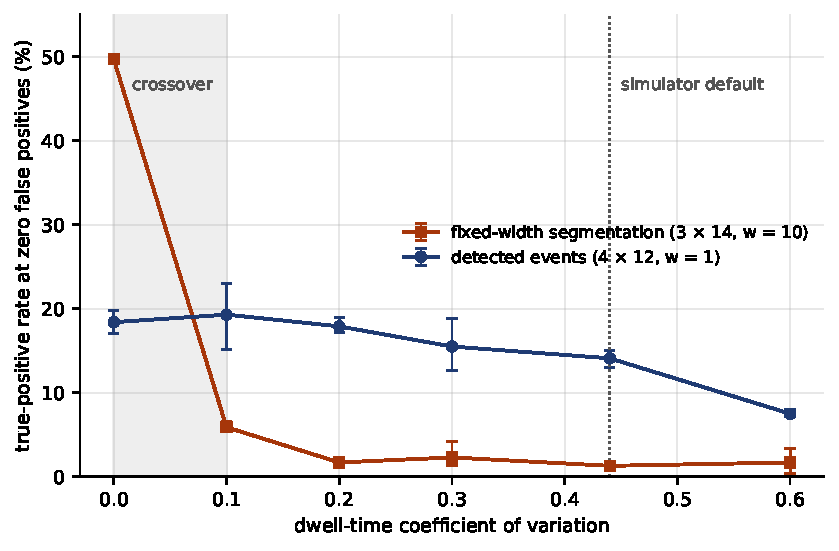
\includegraphics[width=0.82\linewidth]{figures/fig6-1-dwell-crossover.pdf}
\caption{True-positive rate at zero false positives against dwell-time CV for the two segmentation
configurations. Bars span the observed range over three seeds. The shaded band marks the interval
in which the two curves cross; the dotted line marks Squigulator's default dispersion.}
\label{fig:crossover}
\end{figure}

The two arms exchange order between CV~0 and CV 0.10. The replicate ranges do not overlap at any
dispersion tested: at CV~0 the lowest fixed-width replicate, 49.2, exceeds the highest detected
replicate, 19.8, and at every non-zero dispersion the highest fixed-width replicate falls below the
lowest detected one. The order therefore holds in every seed and not only in the means.

The consequence is for configuration selection. An evaluation conducted at CV~0 selects the
fixed-width arm, which leads by 2.7-fold there and trails by 10.8-fold at CV 0.44. This is not an
error of the kind that more data would correct, because every measurement available at CV~0
supports it. The fixed-width arm is not a published method, and the finding concerns the choice
between two configurations of one pipeline under a mis-specified evaluation.
Section~\ref{sec:bound} shows that it does not extend to the method class.

\subsection{A published mapper does not reverse}\label{sec:bound}

At its default, $w = 0$, RawHash2's correct-mapping rate goes from 95.0\% at CV~0 to 92.0\% at
CV 0.60, a loss of 3.0 points, with no crossover and no collapse (Table~\ref{tab:rawhash},
Figure~\ref{fig:rawhash}). The sensitivity found in Section~\ref{sec:reversal} is therefore a
property of fixed-width segmentation and not of quantised-event matching, and a developer
evaluating RawHash2 at constant dwell would reach the same conclusion as one evaluating it at
realistic dispersion. With sketching enabled the decline is steeper, 8.4 points at $w = 5$ (90.0
to 81.6) and 11.2 at $w = 10$ (82.2 to 71.0), which is the subject of
Section~\ref{sec:minimizer}.

\begin{table}[t]
\centering
\caption{RawHash2 across the dwell sweep: percentage of on-target reads correctly mapped and
percentage of control reads mapped at all, by minimizer window $w$. One seed per cell, 500 reads
per set.}
\label{tab:rawhash}
\begin{tabular}{llcccccc}
\toprule
 & & \multicolumn{6}{c}{Dwell CV} \\
\cmidrule(lr){3-8}
Rate & $w$ & 0.00 & 0.10 & 0.20 & 0.30 & 0.44 & 0.60 \\
\midrule
Correct & 0 & 95.0 & 95.2 & 94.6 & 94.2 & 92.4 & 92.0 \\
Correct & 5 & 90.0 & 88.8 & 89.4 & 88.0 & 85.2 & 81.6 \\
Correct & 10 & 82.2 & 82.2 & 82.2 & 79.2 & 77.2 & 71.0 \\
\midrule
False-mapped & 0 & 9.6 & 9.8 & 8.4 & 9.0 & 8.4 & 8.4 \\
False-mapped & 5 & 10.2 & 11.2 & 10.2 & 9.8 & 8.2 & 10.4 \\
False-mapped & 10 & 14.8 & 12.8 & 11.2 & 13.4 & 13.8 & 15.2 \\
\bottomrule
\end{tabular}
\end{table}

\begin{figure}[t]
\centering
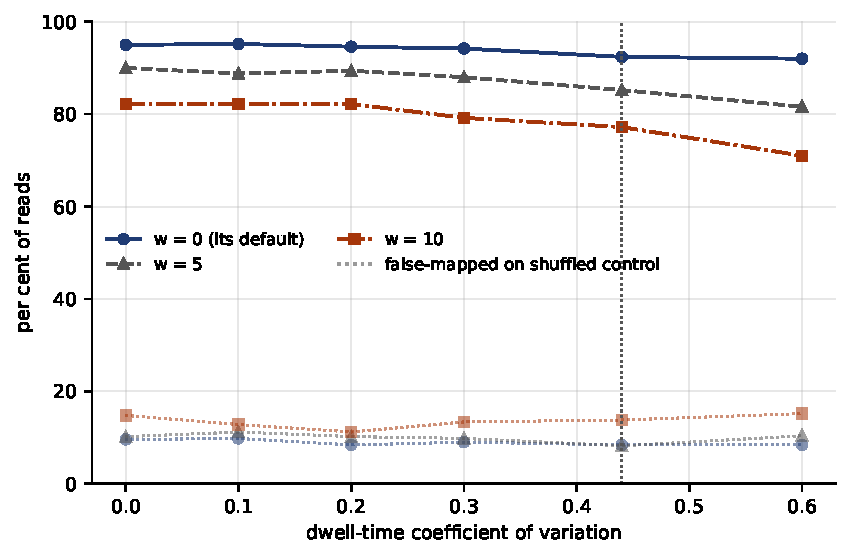
\includegraphics[width=0.82\linewidth]{figures/fig6-2-rawhash-dwell.pdf}
\caption{RawHash2 under the dwell sweep. Solid, dashed and dash-dotted lines: percentage of
on-target reads correctly mapped, by minimizer window. Dotted lines: percentage of control reads mapped. The
default operating point is not zero-false-positive, so these rates are not level-comparable with
Figure~\ref{fig:crossover}.}
\label{fig:rawhash}
\end{figure}

The response to dispersion is visible in the encoding before any seeding or chaining
(Table~\ref{tab:agreement}). RawHash2's per-event agreement is 0.913 at CV~0 and 0.911 at CV 0.44,
and that of the detected arm 0.797 and 0.783. The fixed-width segmentation's agreement falls from
0.793 to 0.648, and its indel fraction rises 2.8-fold, from 0.073 to 0.208. RawHash2's indel
fraction also rises, from 0.055 to 0.092, without a corresponding loss of agreement. Both
segmenters that detect level changes thus have dispersion-invariant agreement, and the one that
segments by time does not. These are two dwell levels, 200 reads and one seed
(Section~\ref{sec:limitations}).

\begin{table}[t]
\centering
\caption{Per-event agreement and indel fraction between reference and query symbol sequences, one
estimator applied to both systems, 200 reads per cell, one seed.}
\label{tab:agreement}
\begin{tabular}{llccc}
\toprule
System & Segmentation & Dwell CV & Agreement & Indel fraction \\
\midrule
This pipeline & fixed-width & 0.00 & 0.793 & 0.073 \\
This pipeline & fixed-width & 0.44 & 0.648 & 0.208 \\
This pipeline & detected & 0.00 & 0.797 & 0.170 \\
This pipeline & detected & 0.44 & 0.783 & 0.196 \\
RawHash2 & own, with merging & 0.00 & 0.913 & 0.055 \\
RawHash2 & own, with merging & 0.44 & 0.911 & 0.092 \\
\bottomrule
\end{tabular}
\end{table}

\subsection{The cost of minimizer sketching depends on dwell dispersion}\label{sec:minimizer}

Table~\ref{tab:penalty} and Figure~\ref{fig:penalty} give the accuracy cost of sketching, the
correct-mapping rate at $w = 0$ minus that at a larger window, in percentage points. At $w = 10$
the cost is 12.8 points at CV~0 and 21.0 at CV 0.60, an increase of 8.2 points, or 64\%. At CV 0.60
sketching at $w = 10$ also raises the false-mapping rate on the control from 8.4\% to 15.2\%, so
both error types worsen together. At $w = 5$ the cost goes from 5.0 to 10.4 points over the same
range.

\begin{table}[t]
\centering
\caption{Accuracy cost of minimizer sketching in RawHash2, $w = 0$ minus the stated window, in
percentage points of correctly mapped reads, from Table~\ref{tab:rawhash}.}
\label{tab:penalty}
\begin{tabular}{lcccccc}
\toprule
Window & 0.00 & 0.10 & 0.20 & 0.30 & 0.44 & 0.60 \\
\midrule
$w = 5$ & 5.0 & 6.4 & 5.2 & 6.2 & 7.2 & 10.4 \\
$w = 10$ & 12.8 & 13.0 & 12.4 & 15.0 & 15.2 & 21.0 \\
\bottomrule
\end{tabular}
\end{table}

\begin{figure}[t]
\centering
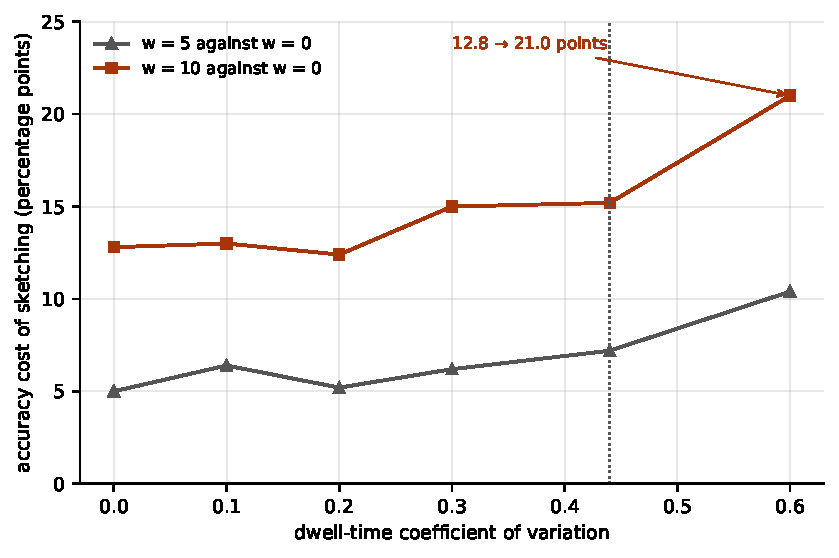
\includegraphics[width=0.82\linewidth]{figures/fig6-3-minimizer-penalty.pdf}
\caption{Accuracy cost of minimizer sketching in RawHash2 against dwell-time CV, for windows 5 and
10 relative to window 0. The dotted line marks Squigulator's default dispersion.}
\label{fig:penalty}
\end{figure}

\paragraph{The growth is not monotone, and the claim is limited accordingly.} At $w = 10$ the
series dips by 0.6 points at CV 0.20, from 13.0 to 12.4. Each cell is one seed. As a scale for
single-cell variation, the three-seed range of the default configuration at CV 0.44 is 1.2 points
(91.2 to 92.4), and a cost is a difference of two such cells. A 0.6-point change is within that
scale and an 8.2-point change is not. The claim made is that the cost is substantially larger at
the top of the range than at the bottom, not that it rises at every step.

\paragraph{What is known and what is added.} RawHash2 ships with sketching disabled to obtain its
highest accuracy, and reports that its minimizer mode maps with accuracy similar to the default
except on the human genome, at higher throughput \citep{firtina2024rawhash2}. That a trade-off
exists is therefore known and documented. What the sweep adds is that its accuracy side is a
function of dispersion. A window chosen from a comparison at one dispersion carries a different
cost at another, and a comparison on constant-dwell signal understates it.

\paragraph{A candidate mechanism, not isolated.} A minimizer is the key of lowest rank within a
window of consecutive keys \citep{roberts2004minimizers}. A displaced event boundary changes the
quantised values of the keys that overlap it and can therefore change which key in a window
attains the minimum, so that reference and query select different keys even where both would
match individually. This requires boundaries to move. At constant dwell the cost reflects only the
seeds that sketching discards; the increment above it is consistent with the mechanism, which
would be demonstrated by recording which keys each side selects, and that was not done.

\subsection{Icarust emits constant dwell, and a patch that removes the restriction}\label{sec:icarust}

Icarust's signal loop emits \texttt{samples\_per\_base} samples for every k-mer, and a source
comment notes that the count could instead be derived from the profile's dwell mean. Its output is
therefore the CV = 0 case exactly, and no configuration of the stock simulator produces
time-domain noise.

The patch in \file{third_party_patches/icarust-dwell-variability.patch} reads a CV from the
environment variable \texttt{ICARUST\_DWELL\_CV} and draws each k-mer's dwell from a lognormal
distribution about \texttt{samples\_per\_base}, with $\sigma^2 = \ln(1 + \mathrm{CV}^2)$ and
$\mu = \ln(\texttt{samples\_per\_base}) - \sigma^2/2$, so that the mean before rounding equals
\texttt{samples\_per\_base} and the CV equals the requested value. Each draw is rounded and clamped
to at least 1 sample, since a k-mer contributing nothing is a skip, which is a different
phenomenon, and to at most 8 times nominal, beyond which a hold is a pore block rather than a
dwell. Unset or 0, the variable reproduces the stock behaviour exactly, so existing results are
unaffected. An environment variable keeps the change minimal and revertible; a version offered
upstream should read the value from the sample profile.

% provisional:begin
\subsection{Secondary observations not backed by a captured run\texorpdfstring{\prov}{}}\label{sec:secondary}

The three observations in this section were made during development. Each rests in part on a
measurement for which no run output was captured. Those values are marked with a dagger; none of
them is used in any claim in Sections~\ref{sec:reversal} to~\ref{sec:icarust} or in the Abstract, and the
verification script lists each as outstanding.

\paragraph{Live accept rates against Icarust.} With the same client, reference and run length, the
fixed-width arm accepted 43.5\%\prov{} of reads and the detected arm 9.6\%\prov{} against stock
Icarust, and 0.5\%\prov{} and 9.6\%\prov{} against the patched simulator at CV 0.35. Taken at face
value, stock Icarust reports the fixed-width arm as 4.5-fold\prov{} better, and the patched
simulator reverses the order, which is the reversal of Section~\ref{sec:reversal} observed on the
live interface. These are accept rates on the live loop and are not comparable with the offline
TPRs of Table~\ref{tab:ours}. Re-running stock and patched Icarust against the client would settle
them.

\paragraph{Calibration target for event detection.} The calibrated detector, threshold 3.0, emits
1562 events per on-target read at CV 0.44, against an ideal of approximately 2000, one event per
base, which is 21.9\% under-segmentation; seed 42 gives 14.2\% TPR in the captured log. In a
development run that was not captured, threshold 2.0 gave 2017\prov{} events per read, close to the
ideal, and 2.0\%\prov{} TPR, 7.1-fold\prov{} lower. An argument offered during development
attributed the difference to frame displacement: a spurious boundary shifts every later key in the
read. That argument does not distinguish the two error types, because a missed boundary removes an
event and shifts every later event index by one exactly as a spurious boundary adds one. A
sufficient explanation is simpler. The event count measures net error, insertions minus deletions,
and is blind to errors that cancel, so a detector that emits the ideal number of events may still
place many boundaries wrongly. The recommendation that follows does not depend on the uncaptured
values: calibrate a detector against agreement or indel fraction (Section~\ref{sec:agreement}), not
against its event count.

\paragraph{Calibration transfer between generators.} A detector threshold calibrated against signal
from a generator written for this project, applied unchanged to Squigulator signal, gave
0.6\%\prov{} TPR at CV~0, where the Squigulator-calibrated detector gives 18.4\% [17.0--19.8], a
30.7-fold\prov{} difference. The two generators differ in their amplitude-noise models, and the
detector threshold is a t-statistic whose operating point depends on that model. Whatever the
magnitude, a result obtained with event detection is interpretable only together with a statement
of how the detector was calibrated and on what signal.
% provisional:end

% ---------------------------------------------------------------------------------------
\section{Discussion}\label{sec:discussion}

The sweep makes visible a variable that a point evaluation holds fixed at an unknown value, and in
the two cases measured here the variable decides the outcome. In Section~\ref{sec:reversal} it
decides which of two configurations is better; in Section~\ref{sec:minimizer} it decides how much a
documented trade-off costs. Neither result depends on the authors' pipeline being accurate, since
the first concerns the relative order of two configurations and the second is measured on
RawHash2.

We draw six recommendations for evaluating raw-signal methods.

\begin{enumerate}
  \item \textbf{Report dispersion with accuracy.} For simulated signal, report the generator's
    dwell parameters. For real signal, report an estimate of dwell dispersion, which could be
    obtained from basecaller move tables, since these record the samples assigned to each base.
  \item \textbf{Report a sweep, not a point,} for any method or parameter that depends on
    segmentation.
  \item \textbf{Compare configurations at the dispersion of the intended data.} A comparison at
    CV~0 can reverse a ranking (Section~\ref{sec:reversal}).
  \item \textbf{Treat the sketching window as dispersion-dependent,} and measure its cost at the
    dispersion of the intended data (Section~\ref{sec:minimizer}).
  \item \textbf{State the calibration target and calibration signal of any event detector,} and
    calibrate against agreement rather than event count (Section~\ref{sec:secondary}).
  \item \textbf{Test read-until clients against a simulator with a dwell model}
    (Section~\ref{sec:icarust}).
\end{enumerate}

The sweep is complementary to existing benchmarks. RawBench varies the components of the pipeline
on fixed data; the sweep varies one property of the data with the pipeline fixed, and adding a
simulated-dispersion axis to a modular benchmark would combine the two. It is equally a way to
quantify methods that correct signal before segmentation: the benefit of a correction such as
CRANE could be reported as a function of the noise source it addresses rather than at one point.
Any pipeline that builds keys from consecutive events, whether by hashing quantised values or by
seeding on event vectors, is exposed to boundary placement in the way Section~\ref{sec:minimizer}
describes, and the sweep is an inexpensive way to measure that exposure.

% ---------------------------------------------------------------------------------------
\section{Limitations}\label{sec:limitations}

\textit{One reference and one profile.} All figures derive from a 20~Mb prefix of one human
chromosome under one R10.4 profile. Reference size affects specificity and hence absolute rates;
the claim is the shape of the response to dispersion, and it has not been tested on a second
reference.

\textit{Simulated signal only.} The mapping from Squigulator's dwell parameter to the dispersion of
any particular device or run is not established here. Measuring the empirical dispersion of a
public dataset and marking it on the axis is the most direct extension.

\textit{Replication.} The RawHash2 dwell $\times$ window grid is one seed per cell. Its default
configuration is replicated at one dwell level, which provides the scale used in
Section~\ref{sec:minimizer} but not a per-cell interval.

\textit{Mechanisms.} The minimizer mechanism of Section~\ref{sec:minimizer} is consistent with the
data and not isolated. The agreement measurement of Section~\ref{sec:agreement} covers two dwell
levels, 200 reads and one seed.

\textit{Absolute level of the detected arm.} The detected configuration's indel fraction is 0.170
already at CV~0, where there is no timing noise to explain it, which indicates a structural
mismatch between this pipeline's reference and query encodings. It lowers that arm's absolute TPR,
and it is one reason we draw only comparisons of shape.

\textit{Operating points.} The two systems are measured at different operating points, zero false
positives for the authors' pipeline and RawHash2's default for RawHash2.

\textit{Scope of the reversal.} The fixed-width arm is a configuration of the authors' pipeline. No
published tool's evaluation is claimed to be wrong.

% ---------------------------------------------------------------------------------------
\section{Conclusion}\label{sec:conclusion}

Dwell-time dispersion is a signal property that Squigulator exposes as a parameter and that
published evaluations of raw-signal mappers do not vary. Sweeping it, with a composition-matched
control and three replicates, shows that an evaluation at constant dwell can select a segmentation
configuration that is 10.8-fold worse at realistic dispersion, and that the accuracy cost of
minimizer sketching in RawHash2 rises from 12.8 to 21.0 points over the range swept. The first
result is bounded by RawHash2's flat response and the second is measured on it. Both follow from
holding fixed a variable that evaluation can move, and both are avoided by reporting accuracy as a
function of it.

\section*{Funding}
[Funding statement to be completed by the authors before submission.]

\section*{Conflict of interest}
None declared.

\section*{Data availability}
All result files, raw logs, the sweep harness, the figure generator, the Icarust and RawHash2
patches and the verification script are in the repository given under Availability and
implementation.

\nolinenumbers
\bibliographystyle{plainnat}
\bibliography{refs}

\end{document}
